
\begin{abstract}
\noindent We present an variational algorithm to solve the \emph{inverse problem} for iterated function systems (IFS). The central idea is to cast the IFS as an generalization of a mixture of of Gaussians model, and to treat the particular sequence of components that leads to a particular point as a latent variable. If we are given such a \emph{code} for each point in the data, we know which points in the dataset should map to one another under the transformations of the IFS, allowing us to reconstruct the transformations. Given the transformations, it is easy find out which sequence of transformations is is most likely for each data point. Iterating these two steps provides us with a basic algorithm to fit an IFS model to data. The variational Bayes framework allows us take additional factors, such as depths, and affine transformations of the data into account, so that our model also functions as a generalizatin of the mixture of Gaussians model.
\end{abstract}
\section{Introduction}
\pb{Briefly: importance of fractals, inverse problem.}

\pb{Iterated Function Systems.}

\pb{Idea behind our approach. EM principle, using variational Bayes.}

\subsection{Preliminaries}
We will deal with datasets which are a set of points $\{x_1, \ldots, x_n\}$ with $x_i \in \mathbb{R}^D$.

Let $F_{t, R}(y) = t + Rx$ be an affine transformation represented by a vector $t$ and a matrix $R$. If $X ~ \cN(\mu, \Sigma)$, then $F_{t, R}(Y) ~ \cN(t + R\mu, R\Sigma R^T)$. Specifically this means that if we take the standard multivariate normal $\cN_0 = \cN(0, I)$ as  canonical source, we can represent every multivariate normal $\langle \mu, \Sigma \rangle$ by an affine transformation $\langle t, R \rangle$ with $t = \mu$, $\Sigma = RR^T$. It also tells us that sampling from $\cN_0$ and applying a series of affine transformations is equivalent to sampling from a particular MVN.

\paragraph{Variational Bayes} Let $x$ be the observed data of a problem, for which we have a model, and let $z$ be the latent variables of the model. If the model has any parameters, we place priors on them so that we can consider them latent variables, and absorb them into $z$ The variational Bayes approach attempts to approximate the distribution $p(z \mid x)$ using a \emph{variational distribution} $q(z)$. We assume that $z$ can be split into subsets $z_1, \ldots, z_m$, for which $q$ factorizes:
\[
q(z) = \prod_i q_i(z_i)
\]
A central result in variational Bayes is that the optimum for each factor is given by:
\begin{equation}
q^*_i(z_i) = \langle \ln p(x, z)\rangle_{/i} + \text {const} \p \label{line:var-bayes}
\end{equation}
Where $\langle \ln p(x, z) \rangle_{/i} = \sum \prod_{j = {1, \ldots, m}/i} q_j(z_j) ln p(x, z)$ with the sum over all values of all $z_j$ except $z_i$. That is, it represents the expectation with respect to all latent variable factors except $z_i$. 

Usually, the values of these optimal factors have cyclical dependencies, which means that we cannot compute $q^*$ directly. We can, however, search for a local optimum by iteration: we start with some initial value, and use (\ref{line:var-bayes}) to compute new values for each factor based on those of the previous generation.  

\section{The IFS model}

\begin{figure*}[t]
  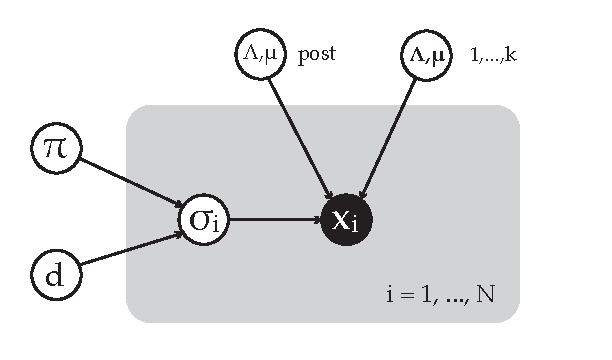
\includegraphics[width=\textwidth]{./images/factor-graph.pdf}
  \caption{A graphical model, illustrating the components of the IFS model. The gray box is a plate, representing a repetition of the nodes inside the box for each datapoint. The black node represents the observed data.}
  \label{figure:ifs-diagram}
\end{figure*}

The complete IFS model is illustrated in Figure~\ref{figure:ifs-diagram}. If contains the following components:
\begin{description}
\item[the component weights $\pi$] This is a vector of $k$ nonnegative real values, with $\sum_i \pi_i = 1$. Each weight determines the probability of its associated component being chosen at each iteration of the IFS.
\item[the depth $d$] The number of times the IFS is iterated.
\item[the components $\bm = \{\mu_1, \ldots, \mu_k\}$, $\bD = \{\Lambda_1, \ldots, \Lambda_k\}$] The means and precision matrices for the $k$ components. 
\item[The post-transformation $\mu_\text{post}$, $\Lambda_\text{post}$] The parameters for a single post-transformation. To see why this is necessary, consider the Koch curve in Ficgure~\ref{figure{fractals}}. While a dataset sampled from this measure can be prefectly represented by an IFS, it is slighty off-center. If this were real dataset, it might be mean-centered instead, in which case no IFS would fit. Unlike the mixture of Gaussians model, an IFS cannot be translated by a straightforward change of the parameters,a nd as the Koch curve shows, simple solutions like mean-centering the data do not always solve the problem. For this reason, we add a single post-transformation into the model, to allow for any simple, affine transformations to the final limit measure. This factor has the additional advantage that at $d = 0$, the model collapses to a single MVN distribution.
\item[The transformation sequence $\sigma_i$] For each data point $x_i$, we have a sequence of length $d$ representing the sequence of component-transformations we need to apply to a point sampled from $\cN_\text{pre}$ to get the final point sampled from the limit measure of the IFS. 
\item[The data $x_i$] This is the point after the post-transformation is applied: ie. the observed data.
\end{description}

The sampling procedure modeled 

This gives us the joint distribution $p(\bs{x}, \bs{\sigma}, \mu_\text{pre}, \Lambda_\text{pre}, \bm, \bD, \mu_\text{post}, \Lambda_\text{post}, \pi, d)$ which factorizes as follows:
\begin{align}
p(&\bs{x}, \bs{x'}, \bs{\sigma}, \mu_\text{pre}, \Lambda_\text{pre}, \bm, \bD, \mu_\text{post}, \Lambda_\text{post}, \pi, d) \notag\\ 
=\;& p(\mathbf{x} \mid \mathbf{x'}, \mu_\text{post}, \Lambda_\text{post}) \; p(\mu_\text{post}, \Lambda_\text{post}) \notag\\
& p(\mathbf{x'} \mid \bs{\sigma}, \bm, \bD, \mu_\text{pre}, \Lambda_\text{pre}) \notag\\
& p(\mathbf{\sigma} \mid \pi, d) \; p(\pi) \; p(d) \notag\\
& \prod_i p(\mu_i, \Lambda_i) \p \label{line:factorization}\\
\end{align}

We use the following priors:
\begin{align*}
p(\pi) &= \text{Dir}(\bs{\alpha}_0) \\
p(d) &= {\cal U}(0, d_\text{max}) \\
p(\mu, \Lambda) &= p(\mu \mid \Lambda) p(\Lambda) = \cN(\mu \mid \bs{m}_0, (\beta_0\Lambda)^{-1}) {\cal W}(\Lambda \mid \bs{W}_0, \nu_0) \p
\end{align*}

Where the last line, a Gaussian-Wishart prior, applies to each pair of $\mu$ and $\Lambda$.

\subsection{The Inference algorithm for IFS models}
We assume the following factorization for our variational distribution to approximate  $p(\bs{z}|\bs{x})$:
\begin{align*}
q(& \mu_\text{pre}, \Lambda_\text{pre}, \bm, \bD, \bs{\sigma}, \pi, d) \\ 
=\;&  q_{\mu_\text{pre}, \Lambda_\text{pre}}(\mu_\text{pre}, \Lambda_\text{pre}) \; q_{\bm, \bD}(\bm, \bD)\; q_{\bs{\sigma}}(\bs{\sigma}) \; q_{\pi, d}(\pi, d) \p \\
\end{align*}
For the sake of clarity, we will omit the subscripts from the factors in the following.

\subsection{Update rules}

\paragraph{Responsibilities}

The derivation of the update rule for the responsibilities, ie. $q_{bs{\sigma}}^{n}(\bs{\sigma})$ takes the same form as the case for the mixture of Gaussians model \cite{}, since our model is essentially a mixture of $k^d$ Gaussians. Note that we can visualize $q(\bs{sigma})$ as a large matrix with $n$ rows and $2^d$ columns.

We have:
\begin{align*}
q^n(\bs{\sigma}) &= \langle \ln p(x, \bm, \bD, \mu', \Lambda', \bs{\sigma}, \pi, d) \rangle_{\bm, \bD, \mu', \Lambda', \pi, d} + const \p
\end{align*}

We factorize $\ln p(\ldots)$ according to (\ref{line:factorization}), and absorb any terms that don't depend on $\bs{\sigma}$ into the constant:   
\begin{align*}
q^n(\bs{\sigma}) &= \langle \ln p(x \mid \bm, \bD, \mu', \Lambda', \bs{\sigma}) \rangle_{\bm, \bD, \mu', \Lambda'} +  \langle \ln p(\bs{\sigma} \mid \pi, d) \rangle_{\pi, d} + const \p\\
& = 
\end{align*}


\paragraph{Components}

\paragraph{Component weights}

\paragraph{Pre-transformation}

\paragraph{Depth}


\subsection{Results}

\section{The RIFS model}
\paragraph{Random Iterated Function Systems}

\subsection{The Inference algorithm for RIFS models}
\subsection{Results}

\section{Discussion}

\pb{Recap.}
